In the initial docking stage of the IDSITE protocol Glide is used to generate a number of proposed docked conformations for each ligand.
Glide (standard precision) is used to generate a number of different ligand conformations by sampling conformations of freely rotatable bonds and rings.
A bounding box, which will be used for a grid search, is defined centered at the centroid of the ligand with an edge length of 10 angstroms.
Because the crystal structure used for CYP2D6 (PDBID: 2F9Q) does not have a ligand, the centroid of residues Glu216, Asp301, Thr309, and Phe483 was used instead in this case.
Because the steric clashes present in many proposed docked conformations can be relieved using a simple minimization procedure a reduced Van der Waals (VDW) radii were used in the docking stage, and additional filtering of possible high energy conformations was also skipped in order to ensure the greatest diversity of docked poses reached the refinement stage.
The collection of docked poses are then clustered according to the RMSD of the ligand, and each pose is minimized.
The top sixty ranked poses according to the Glide SP metric are retained screened using a number of different criteria.
A hard sphere overlap criteria is used to remove poses with obvious steric clashes which were not removed during the minimization procedure.
A number of other rule based geometric screens are used to remove structures which are unlikely to react.
Structures where:
\begin{enumerate}
\item The distance of the basic nitrogen to the ferryl oxygen is less than 5.0 angstroms;
\item The distance of the basic nitrogen to the negative charged oxygen (in Glu216 or Asp301) is greater than 5.5 angstroms;
\item More than 2 heavy atoms from the ligands are further than 16.0 angstroms away from the heme iron;
\item More than 1 heavy atom from the ligand are closer than 1.0 angstroms to the receptor;
\item More than 6 heavy atoms from the ligand are closer than 1.8 angstroms to the receptor;
\item No heavy atom in the ligand is within 5.0 angstroms to the heme iron;
\end{enumerate}
are removed and the remaining poses are passed on to the first Monte Carlo Minimization refinement stage.

% joe is this far

IDSite uses reduced VDW radii for nonpolar atoms both in the protein receptor and the ligand, so that slight steric clashes are tolerated during the docking stage.
For the protein receptor the VDW scaling factor is fixed at 0.40, while for the ligand, the scaling factor starting from 0.80 is adaptively adjusted until at least 4 valid poses are found.
With highly flexible ligands and relatively high scaling factors, Glide often finds only a handful of valid poses, and even fewer survive after IDSite screening.
However, if the scaling factor is set too low, the docked poses may contain too many serious steric clashes, which can cause problems in the subsequent minimization.
If IDSite fails to find enough valid poses, the scaling factor is adjusted and the number of poses to pass the initial docking phase in Glide is increased accordingly to augment sampling.
Since a typical CYP2D6 substrate forms a highly conserved salt bridge with either Glu216 or Asp301,125 IDSite employs this conserved interaction to reduce the sampling cost of the CYP2D6-docking in the following way: IDSite adds a positional constraint to ensure that the generated poses fulfill at least part of the preferred conserved interactions.
The positional constraint defines a spherical region in the receptor that is within 4.0 angstroms of the center of the Glu216, Asp301, and Ser304 residues (Figure 3.2).
It is required that during docking and post- docking minimization each pose should maintain at least one hydrogen-bond donor inside the spherical region.
If the ligand contains other hydrogen-bond donors except for the basic nitrogen, the constrained docking is likely to generate poses that form hydrogen bonds instead of the salt bridge to Glu216 or Asp301.
However, IDSite is able to distinguish these poses and filter them via an additional salt bridge filter in the pose screening (Table 3.1), so that only the poses with a stable salt bridge are allowed to pass to the refinement stage.

\begin{figure}[h]
\centering
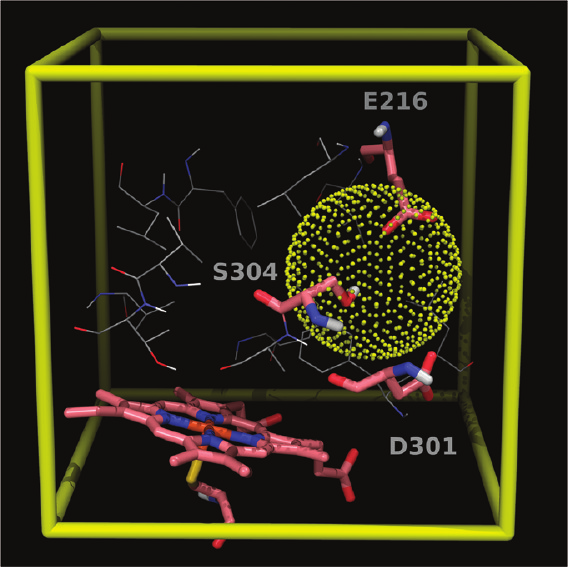
\includegraphics[width=0.35\textwidth]{figures/idsite/glide.png}
\caption{An overview of the entire IDSite procedure.}
\label{fig:idsite_glide}
\end{figure}
